\section{Open Communities}
\begin{comment}
* What is open / what are open communities?
** What's open source/content?
** some projects you may have heard of (Firefox, Wikipedia, etc)
** some you may not have (Wikiotics, CivX, FreeCiv, Civicommons, Sahana, CiviCRM)
** it's not just Linux - a lot of this stuff runs on other platforms too (Windows, Mac, web-based) "no, we are not trying to get you to reinstall your computer" (but if you're interested, we're happy to help)
** the Four Freedoms (made for software)
*** Freedom / friends / ?
** creative commons (made for content)
** it's more than licensing... what's "the open source way," some characteristics of those communities (realtime transparency, etc)
\end{comment}

% I'm going to use a line of comment markers to indicate that there is a new
% frame happening. It will make things a bit a bit easier to read.

%%%%%%%%%%%%%%%%%%%%%%%%%%%

\begin{frame} 
\frametitle{what are open communities?}
% Not always distributed - events.
% Not always volunteers - companies.
% Not always given away - support.
% But it's a good starting place.

\huge
\begin{center}
\begin{minipage}{7cm}
A \alert{distributed} group of \alert{volunteers} committed to \alert{giving away} their efforts.
\end{minipage}
\end{center}

\end{frame} 

%%%%%%%%%%%%%%%%%%%%%%%%%%%

\begin{frame} 
\frametitle{what is the open source way?}
% Applies to projects that aren't software.
% Open government, medicine, etc.
% (opensource.com stories go here)

\huge
\begin{center}
Radically cross-functional,
collaboratively constructed
\alert{realtime transparency}.
\end{center}

\end{frame} 

%%%%%%%%%%%%%%%%%%%%%%%%%%%

\begin{frame} 

% 'T' aligns the top of the columns, 'c' the center.
\begin{columns}[T] 
% ** some you may not have (Wikiotics, CivX, FreeCiv, Civicommons, Sahana, CiviCRM)
\column{1.5in} 
\begin{itemize}
	\item Firefox
	\item Wikipedia
	\item Wikiotics
	\item CivX
	\item FreeCiv
	\item Sahana
\end{itemize}

\column{1.5in} 
% Framebox puts a frame around the image... not what I want here.
%\framebox{
\includegraphics[height=2cm]{images/ff-logo.png}}

\includegraphics[height=2cm]{images/ff-logo.png}
\vspace{1cm}

\includegraphics[height=2cm]{images/wiki-logo.png}
\vspace{1cm}
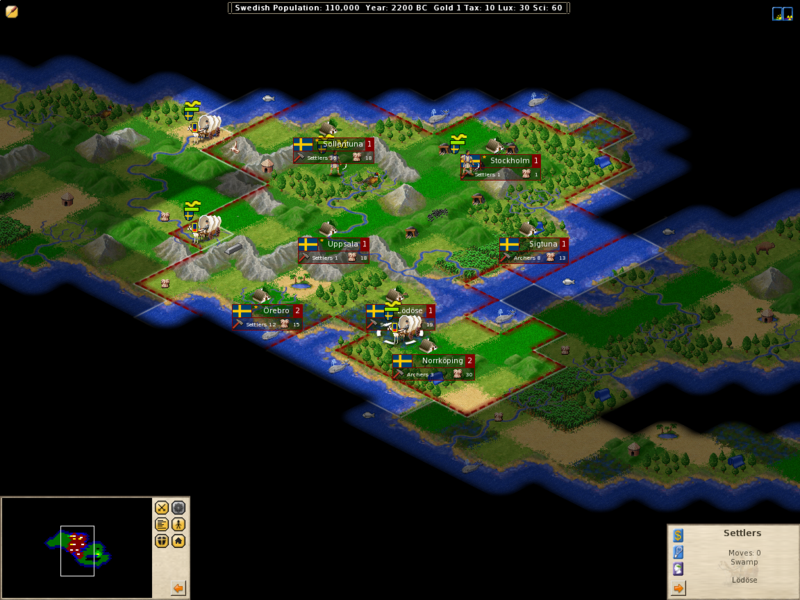
\includegraphics[height=2cm]{images/freeciv-logo.png}
\end{columns}
\end{frame}

%%%%%%%%%%%%%%%%%%%%%%%%%%%

\begin{frame} 
\frametitle{four freedoms}
% Not to be confused with http://en.wikipedia.org/wiki/Four_Freedoms
% which is FDR's famous 1941 State of the Union address on
% freedom of speech and worship, and freedom from want and fear.
%
% Original: http://www.gnu.org/philosophy/free-sw.html
%
% The freedom to run the program, for any purpose (freedom 0).
%
% The freedom to study how the program works, and change it so 
% it does your computing as you wish (freedom 1). Access to the 
% source code is a precondition for this.
% 
% The freedom to redistribute copies so you can help your neighbor 
% (freedom 2).
% 
% The freedom to distribute copies of your modified versions to others
% (freedom 3). By doing this you can give the whole community a chance 
% to benefit from your changes. Access to the source code is a 
% precondition for this.

\huge
\begin{center}
\begin{minipage}{7cm}
\begin{itemize}
	\item Freedom to \alert{use}
	\item Freedom to \alert{change}
	\item Freedom to \alert{share}
	\item Freedom to \alert{share your changes}
\end{itemize}
\end{minipage}
\end{center}

\end{frame} 

%%%%%%%%%%%%%%%%%%%%%%%%%%%
